\section{Versuchsdurchführung}

Zuerst wird überprüft, dass der Winkelmesser korrekt kalibriert ist, indem der Winkelmesser auf etwa 180\textdegree aufgeklappt und auf den Tisch gelegt wird. Wenn er dabei 180\textdegree anzeigt misst der Winkelmesser korrekt. \\
Der Winkel $\alpha$ wird mithilfe einer Winkelmessung $\beta$ zwischen der schiefen Ebene und der Vertikalen gemessenen. Da der vertikale Träger des Gerüsts nicht senkrecht zu der Horizontalen ist, wird der Winkel $\gamma$ gemessenen. Mit \autoref{eq:alpha} wird $\alpha$ berehnet.

\begin{align}
    \alpha = 90^\circ - (\beta - (90^\circ - \gamma))
    \label{eq:alpha}
\end{align}

\begin{figure}[ht]
    \centering
    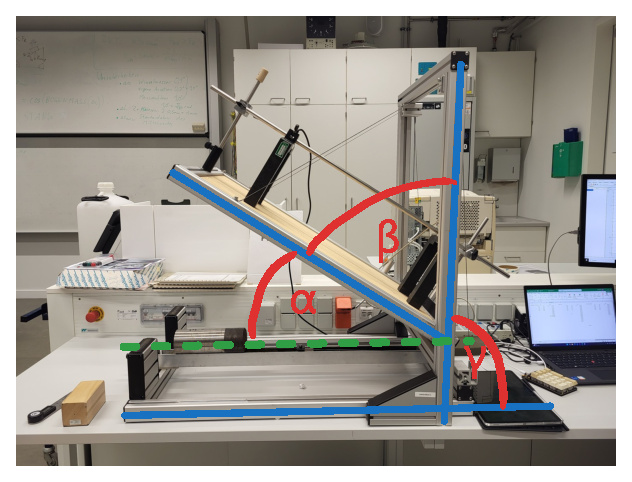
\includegraphics{images/Versuch-Winkel.pdf}
    \caption[Winkelmessung]{Winkel $\alpha$, $\beta$ und $\gamma$}
    \label{fig:Winkelmessung}
\end{figure}

Darauf wird die Länge $l$ zwischen beiden Lichtschranken mit dem Gliedermaßstab gemessen (siehe \autoref{fig:Lichtschranken}).\\

Um $\mu_{HR}$ zu bestimmen wird der Körper am Ende der schiefen Ebene platziert und der Winkel $\alpha$ so lange erhöht, bis der Körper anfängt zu rutschen. Nachdem $\alpha_{max}$ notiert wurde, wird der Körper und der Winkel der schiefen Ebene zurückgesetzt. $\alpha$ wird wieder erhöht bis der Körper anfängt zu rutschen. Das wird für für drei Seiten des Körpers je fünf mal wiederholt.\\
Um $\mu_{GR}$ zu bestimmen wird der Winkel $\alpha$ größer eingestellt als das größte zuvor notierte $\alpha_{max}$ für die jeweilige Seite. Der Körper wird genau so platziert, dass er kurz davor ist die Lichtschranke auszulösen und darauf losgelassen. Die Zeit $t_{mess}$, die der Block braucht um $l$ zurückzulegen, wird notiert und der Würfel wird wieder kurz vor der Lichtschranke platziert. Dies wird für drei der Seiten je zehn mal wiederholt.

\begin{figure}
    \centering
    \begin{tikzpicture}
    \node[anchor=south west,inner sep=0] at (0,0) {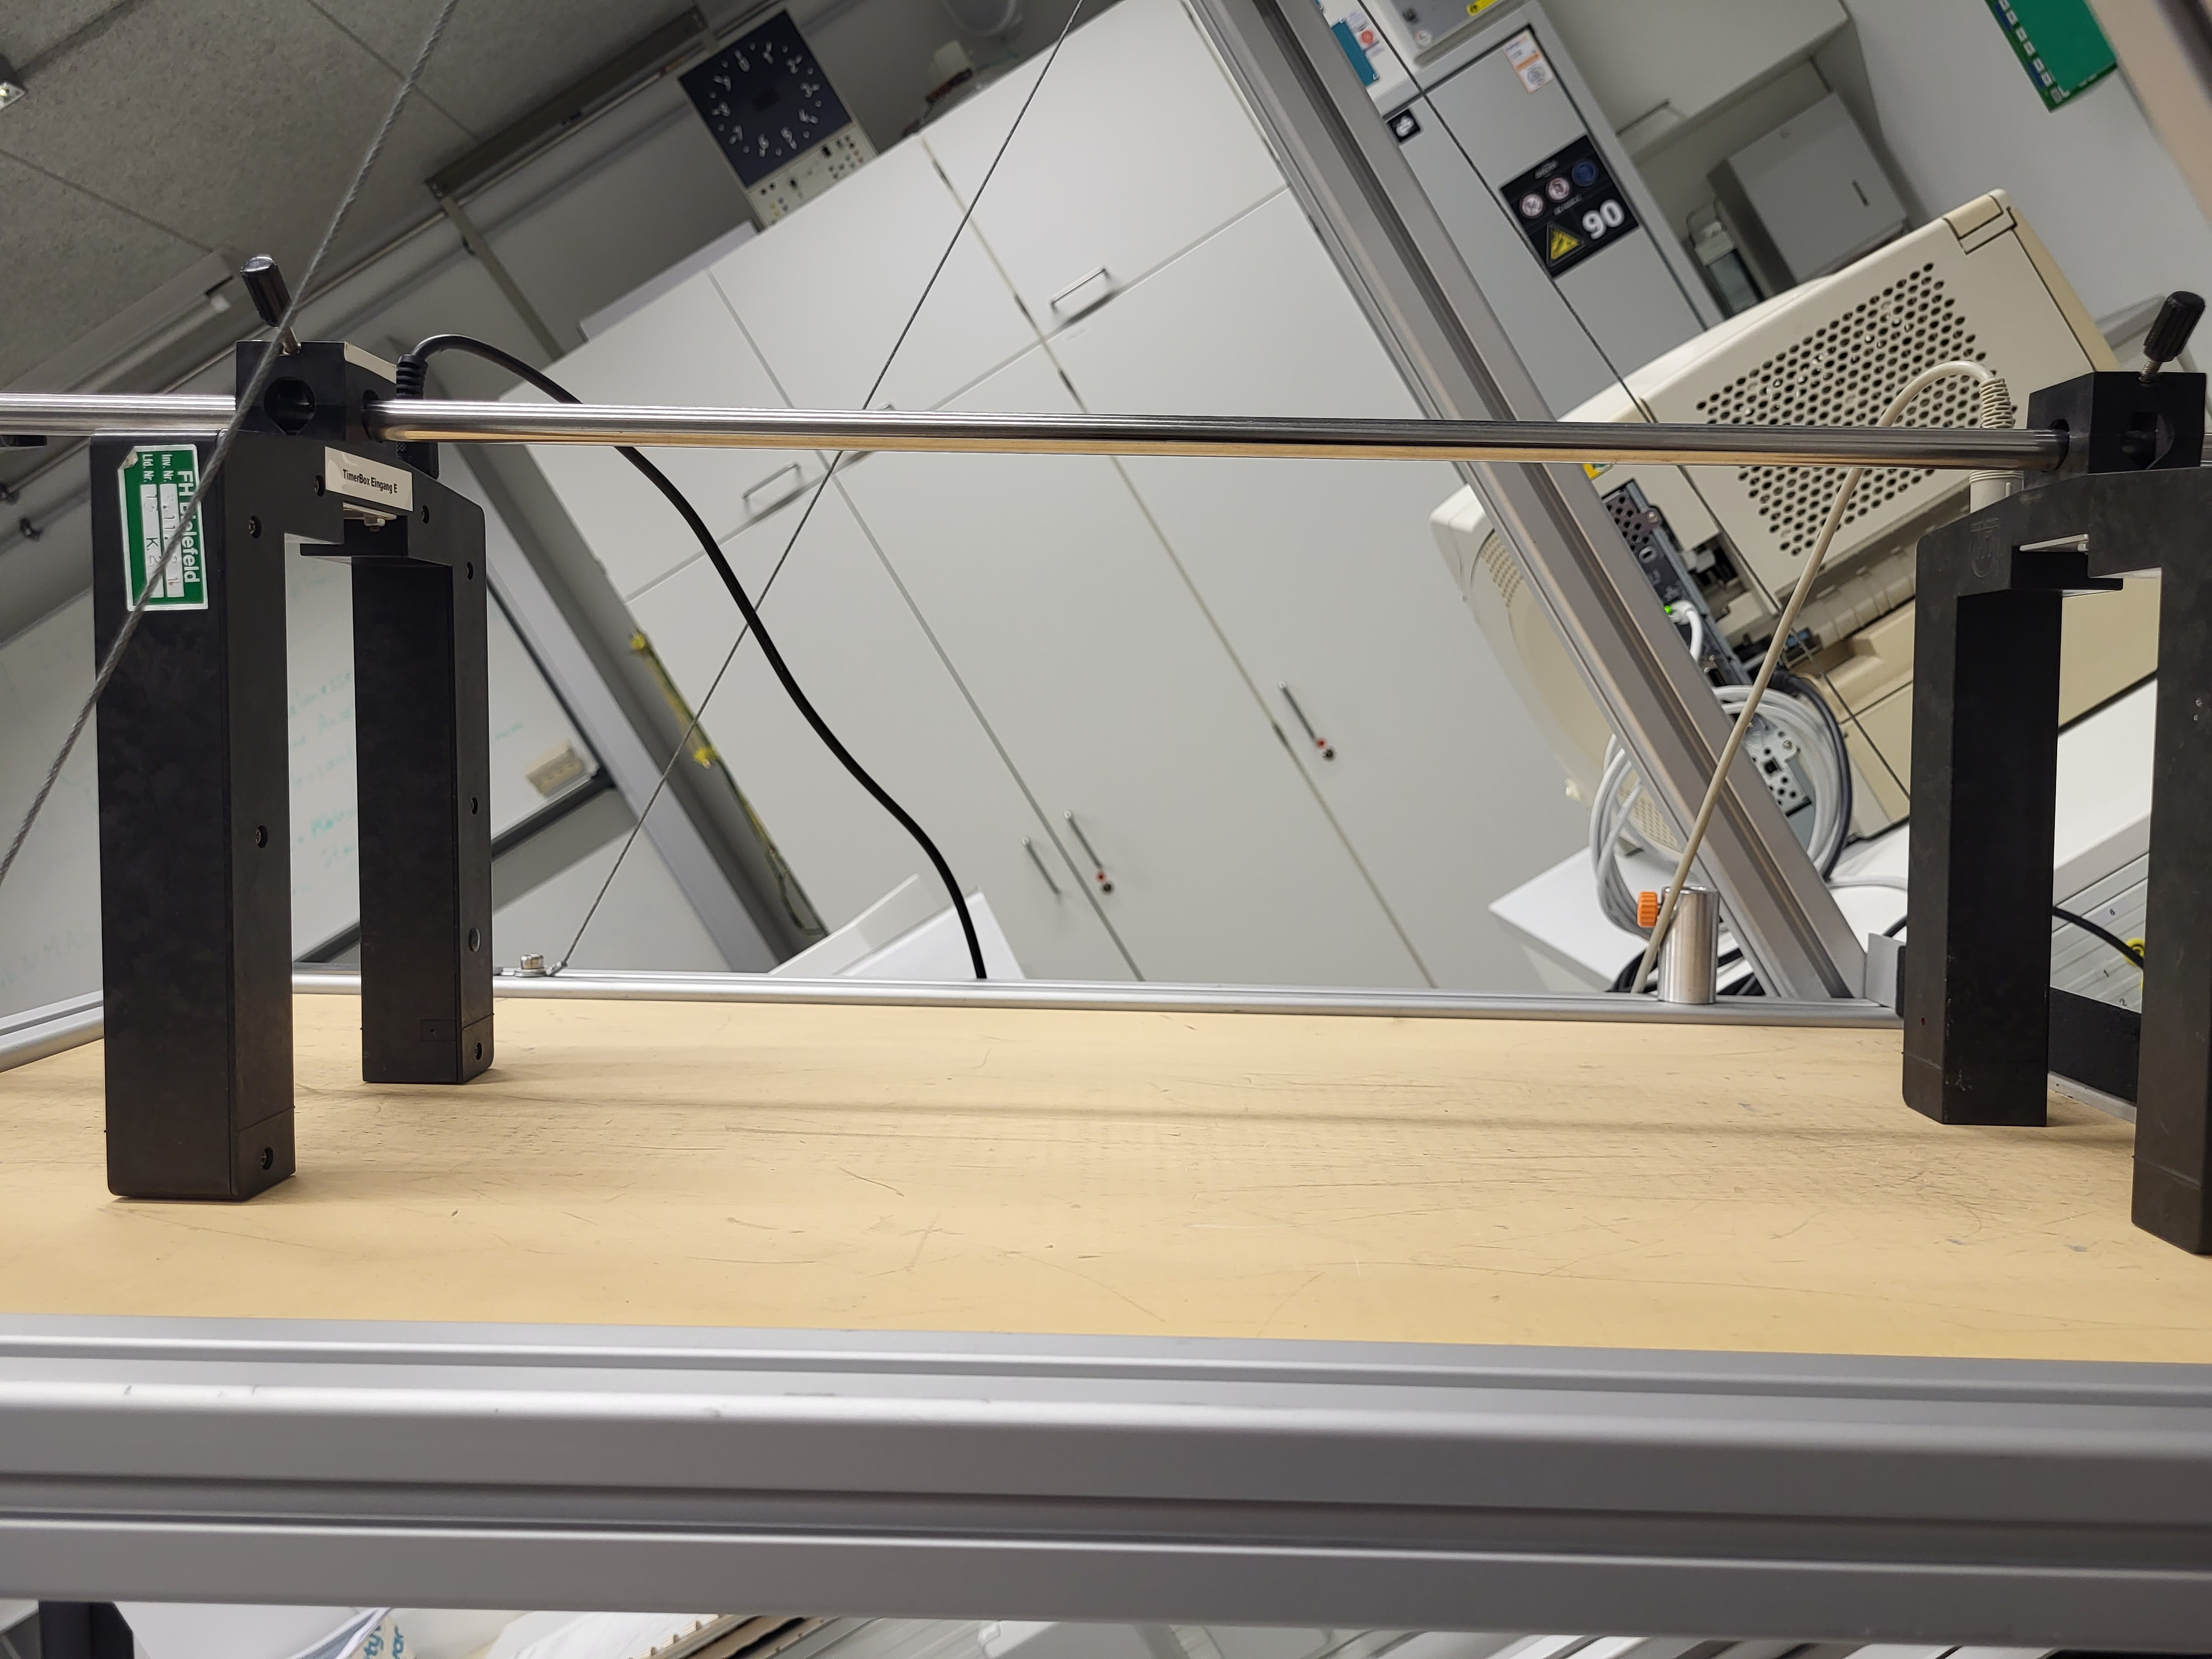
\includegraphics[width=\textwidth/2]{images/Versuch-Lichtschranken.jpg}};
    \draw[red, ultra thick, |-|](3.4/2,4.9/2) -- (15.65/2,4.6/2);
    \draw [red](3.4/4+15.65/4,4.9/4+4.6/4 + 0.5) node {$l$};
\end{tikzpicture}
    \caption[Lichtschranken]{Länge $l$ zwischen den Lichtschranken}
    \label{fig:Lichtschranken}
\end{figure}